\begin{figure}
\def\miny{-2}
\def\maxy{5}
\def\swp #1 {\draw[loosely dashed] (#1,\miny) -- (#1,\maxy);}
\begin{center}
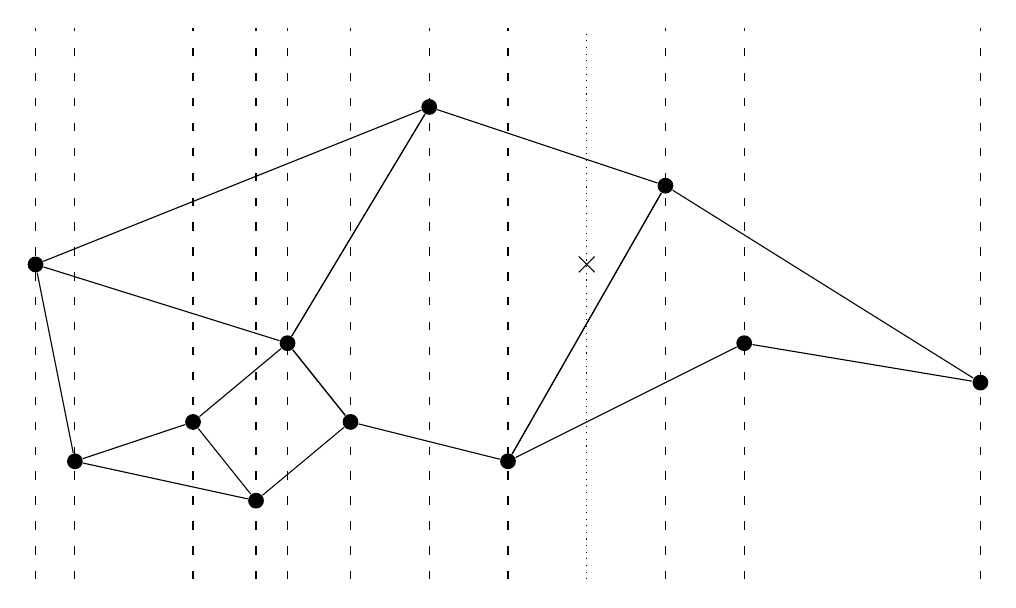
\begin{tikzpicture}[
point/.style={circle, fill=black, inner sep=0pt, minimum width=2mm},
]

\node[point] at (0.2,1) (c) {};
\node[point] at (1,0) (d) {};
\node[point] at (-0.2,-1) (a) {};
\node[point] at (-1,0) (b) {};
\node[point] at (5,3) (e) {};
\node[point] at (2,4) (f) {};
\node[point] at (-3,2) (g) {};
\node[point] at (-2.5,-0.5) (h) {};
\node[point] at (3,-0.5) (i) {};
\node[point] at (9,0.5) (j) {};
\node[point] at (6,1) (k) {};

% Rectangle:
\draw (a) -- (b) -- (c) -- (d) -- (a);

\draw (a) -- (h) -- (b);

\draw (g) -- (c);

\draw (h) -- (g) -- (f) -- (c);

\draw (c) -- (f) -- (e) -- (i) -- (d) -- (c);

\draw (i) -- (k) -- (j) -- (e) -- (i); 

\swp{-3}
\swp{-2.5}
\swp{-1}
\swp{-0.2}
\swp{0.2}
\swp{1}
\swp{2}
\swp{3}
\swp{5}
\swp{6}
\swp{9}

% Cross:
\draw (3.9,1.9) -- (4.1,2.1);
\draw (4.1,1.9) -- (3.9,2.1);
{\draw[dotted] (4,\miny) -- (4,\maxy);}
\end{tikzpicture}
\end{center}
Positions of sweeping line during the run of point-localization algorithm are depicted as dashed lines. Queried point is denoted as a cross. Edges intersecting the dotted line are in the version of $S$ that will be queried.
\caption{Localization of a point}
\end{figure}